\documentclass[conference]{IEEEtran}
\IEEEoverridecommandlockouts

\usepackage[utf8]{inputenc}
\usepackage[portuguese]{babel}
\usepackage{amsmath,amssymb,amsfonts}
\usepackage{graphicx}
\usepackage{textcomp}
\usepackage{xcolor}
\usepackage{float}
\usepackage{url}

\def\BibTeX{{\rm B\kern-.05em{\sc i\kern-.025em b}\kern-.08em T\kern-.1667em\lower.7ex\hbox{E}\kern-.125emX}}

\begin{document}

	\title{Implementação do Perceptron: Avaliação de Desempenho em Problemas de Classificação Binária\\}

	\author{\IEEEauthorblockN{Hebert Alan Kubis}
	\IEEEauthorblockA{\textit{Engenharia Mecatrônica} \\
	\textit{Universidade Federal de Santa Catarina (UFSC)}\\
	Centro Tecnológico de Joinville, Brasil}
	}

	\maketitle

	\begin{abstract}

		Este documento apresenta a implementação em linguagem C de uma rede neural artificial do tipo Perceptron de camada única, desenvolvida para resolver problemas de classificação binária. O algoritmo base foi estruturado de forma genérica, logo não se limita à classificação unicamente binária. A implementação foi testada utilizando uma base de dados gerada sinteticamente para ser linearmente separável e a base de dados Iris, utilizando a metodologia hold-out para validação.

	\end{abstract}

	\begin{IEEEkeywords}

		Perceptron, Inteligência Artificial, Classificação Binária, C, Python.

	\end{IEEEkeywords}

	\section{Introdução}

		O Perceptron é a forma mais simples de rede neural artificial, sendo composto por um único neurônio de saída, e é utilizado para resolver problemas de classificação linearmente separáveis. 

		O algoritmo desenvolvido neste documento implementa o perceptron para classificar dados em duas classes distintas, utilizando a função de ativação em degrau para determinar a saída binária, mas não se limita a isso, podendo ser utilizado para classificação multiclasse com a adição de mais neurônios na saída.

	\section{Metodologia e Configuração da Rede}

		\subsection{Implementação do Motor Neural}

			O Perceptron foi implementado em C, baseando-se no paradigma de programação orientada a objetos, utilizando estruturas para representar os neurônios e, também, para representar a rede como um todo. A implementação inclui a inicialização dos pesos das entradas, o processo de treinamento utilizando o algoritmo de aprendizado supervisionado e a função de ativação para gerar as previsões.

		\subsection{Estratégia de Validação (Hold-out)}

			Para garantir a integridade da avaliação do modelo, adotou-se a metodologia de validação do tipo \textit{Hold-out}. O conjunto de dados original foi segmentado de forma estática na proporção de 2/3 para o subconjunto de Treinamento e 1/3 para o subconjunto de Teste e embaralhado com a função \texttt{rand()} a cada época, sendo a seed redefinida a cada execução do programa. 

			As métricas de avaliação foram calculadas exclusivamente sobre os dados de teste que a rede nunca observou durante o processo de ajuste.

		\subsection{Parâmetros da Rede}

			Para o treinamento do Perceptron, foram definidos os seguintes parâmetros:

			\begin{itemize}
				\item \textbf{Taxa de Aprendizado ($\eta$):} 0.65
				\item \textbf{Critério de Parada:} Número máximo fixo de 100 \textit{epochs}.
				\item \textbf{Função de Ativação:} Função Degrau (0 e 1).
				\item \textbf{Arquitetura:} 1 neurônio de saída.
			\end{itemize}

	\section{Testes e Resultados Computacionais}

		\subsection{Base de Dados Linearmente Separável (2D)}

			O primeiro experimento consistiu na aplicação da rede para segmentar uma base de dados sintética gerada de forma a garantir a separabilidade linear no plano bidimensional. O \textit{dataset} foi balanceado, sendo composto por classes delimitadas em quadrantes opostos. Com esta base bidimensional aplicada ao Perceptron, a fronteira de decisão foi ajustada de forma simples e rápida (já na segunda \textit{epoch}), como mostra a figura \ref{fig:perceptron_decision_boundary}, onde a linha verde tracejada representa a fronteira de decisão ajustada pelo Perceptron.

			\begin{figure}[H]
				\centering
				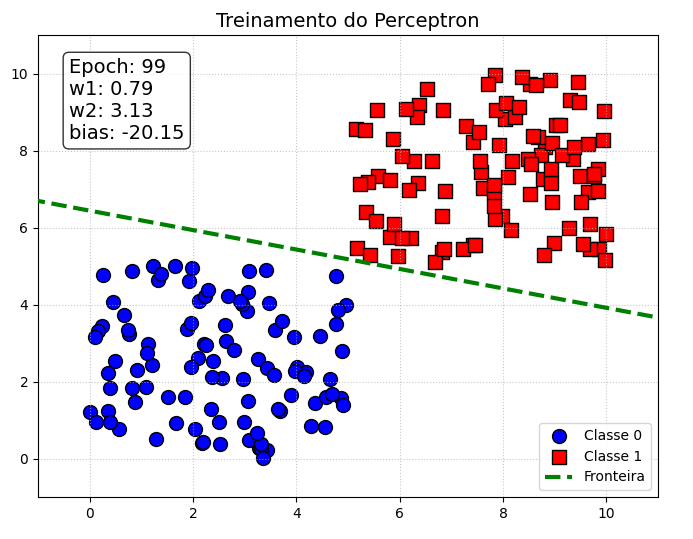
\includegraphics[width=0.35\textwidth]{img/perceptron treinado 2d ls.png}
				\caption{Fronteira de decisão do Perceptron ajustada no plano bidimensional.}
				\label{fig:perceptron_decision_boundary}
			\end{figure}

		\subsection{Desempenho na base linearmente separável}

			Após a execução do algoritmo de treinamento e predição, foram extraídas métricas de avaliação via linguagem Python utilizando a biblioteca Scikit-learn \cite{Scikit-learn} e para visualização foi utilizada a biblioteca Matplotlib \cite{matplotlib}.

			Para este teste, não será mostrado o gráfico de acurácia x época, pois a acurácia atingiu $100\%$ já na segunda época. De todo modo, a matriz de confusão é apresentada na figura \ref{fig:confusion_matrix}, onde pode-se observar que o modelo classificou corretamente todas as amostras, sem apresentar Falsos Positivos ou Falsos Negativos.

			\begin{figure}[H]
				\centering
				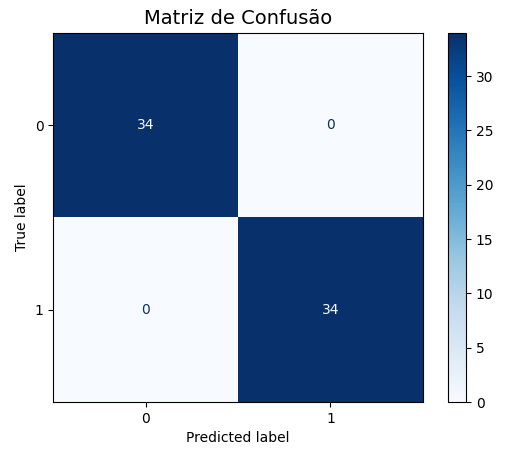
\includegraphics[width=0.35\textwidth]{img/matriz de confusao 2d ls.png}
				\caption{Matriz de Confusão para a base linearmente separável.}
				\label{fig:confusion_matrix}
			\end{figure}

		\subsection{Base de Dados Iris (Versicolor x Virginica)}

			O segundo teste foi realizado na base de dados Iris, utilizando apenas as classes Versicolor e Virginica, classificadas, respectivamente, como 0 e 1, que não são linearmente separáveis, para verificar o comportamento do Perceptron em um cenário onde é impossível convergir. Nesse teste também foi tratada a questão da multidimensionalidade, utilizando as quatro características disponíveis para o treinamento e predição.

		\subsection{Desempenho na base Iris}

			Como a base é multidimensional, os dados analisados não podem ser visualizados de forma espacial direta. Deste modo, o Perceptron será avaliado com base na curva de Acurácia x Época e na matriz de confusão. 

			\begin{figure}[H]
				\centering
				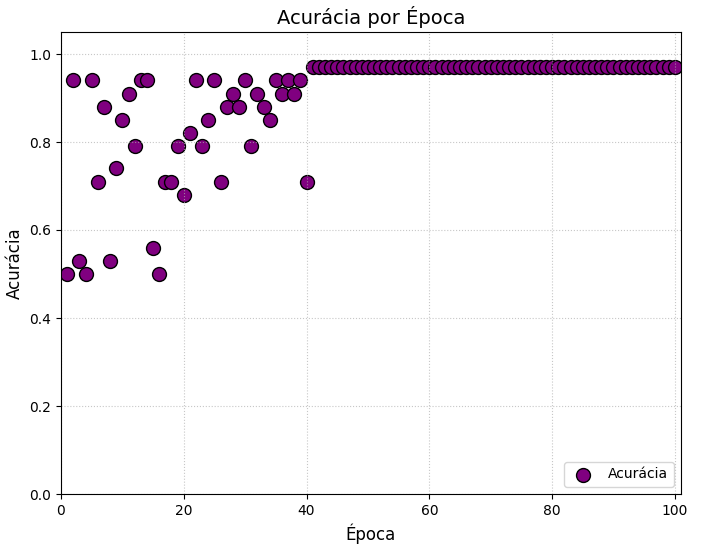
\includegraphics[width=0.35\textwidth]{img/acuracia por epoca iris.png}
				\caption{Curva de Acurácia ao longo das épocas para a base Iris.}
				\label{fig:accuracy_per_epoch_iris}
			\end{figure}

				Na figura \ref{fig:accuracy_per_epoch_iris} é possível visualizar que a acurácia do modelo oscilou bastante durante as primeiras épocas (provavelmente devido à taxa de aprendizado alta utilizada). Contudo, ao atingir o limite de iterações, a precisão da última época computada resultou em $97\%$. É importante destacar que o comportamento esperado para dados não linearmente separáveis é que o modelo oscile indefinidamente, visto que o erro de classificação nunca é zerado e a regra de aprendizado continua forçando atualizações nos pesos. 

				Neste caso específico, a estabilização da curva de acurácia em um patamar alto ocorreu porque os contínuos ajustes da fronteira de decisão não foram grandes o suficiente para alterar a predição das amostras do conjunto de teste. Vale ressaltar que o obstáculo para atingir $100\%$ de acurácia é a limitação matemática fundamental do Perceptron de camada única, que é incapaz de traçar fronteiras de decisão não lineares para contornar a zona de sobreposição entre a Versicolor e a Virginica.

				\begin{figure}[H]
					\centering
					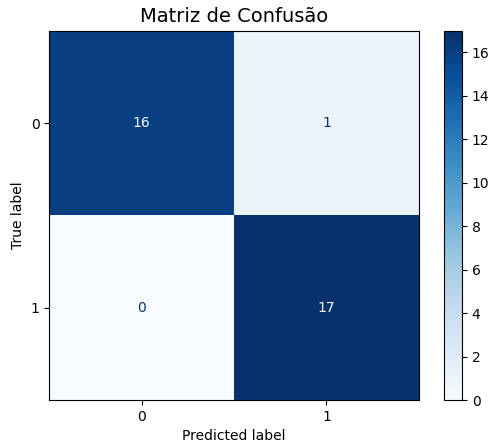
\includegraphics[width=0.35\textwidth]{img/matriz de confusao iris.png}
					\caption{Matriz de Confusão para a base Iris (Versicolor x Virginica).}
					\label{fig:confusion_matrix_iris}
				\end{figure}

				Outra métrica importante para avaliar o desempenho do modelo é a matriz de confusão, apresentada na figura \ref{fig:confusion_matrix_iris}. Nela é possível observar que o modelo classificou uma amostra como Virginica quando na verdade era Versicolor, o que corresponde a um Falso Positivo. Este resultado é coerente com a acurácia de $97\%$ apresentada na curva de acurácia x época, indicando que o modelo teve um desempenho elevado, mas não perfeito, dadas as limitações estruturais da rede frente à sobreposição das classes.

	\section{Conclusão}

		O perceptron implementado em C funcionou conforme o esperado, conseguindo classificar corretamente os dados da base linearmente separável e não convergindo matematicamente para uma solução estática na base Iris. A rede demonstrou o comportamento teórico esperado de oscilação em cenários não separáveis, embora o critério de parada por épocas tenha garantido uma fronteira de decisão com alta taxa de acerto.

	\begin{thebibliography}{00}
		\bibitem{Scikit-learn} sklearn.metrics. Scikit-learn, 2026. Disponível em: \url{https://scikit-learn.org/stable/api/sklearn.metrics.html}. Acesso em: 22 de maio de 2026.
		\bibitem{matplotlib} matplotlib.pyplot. Matplotlib, 2026. Disponível em: \url{https://matplotlib.org/stable/gallery/pyplots/index.html}. Acesso em: 22 de maio de 2026.
		\bibitem{material-aula} Material de aula do curso de Sistemas Inteligentes, ministrado pelo professor Dr. Pablo Andretta Jaskoviak.
	\end{thebibliography}

\end{document}